\documentclass{beamer}

\mode<presentation>
{
  \usetheme{Boadilla}
  \beamertemplatenavigationsymbolsempty
}
\setlength\abovecaptionskip{0pt}

\usepackage{fontspec}
\setmainfont{Liberation Serif}
\setsansfont{Liberation Sans}
\setmonofont{Liberation Mono}

\usepackage{polyglossia}
\setdefaultlanguage[variant=us]{english}

\usepackage{csquotes}

\title[Identifying Woodblocks]{Identifying Woodblocks from the Bukan Collection}
\subtitle{Were some woodblocks the same for multiple editions?\\Were they
  modified in some way?}
\author{Thomas Leyh}
\institute[]{University of Freiburg, Germany}
\date{November 12th, 2019}

\begin{document}
  \begin{frame}
    \titlepage
  \end{frame}

  \begin{frame}
    \frametitle{Bukan Collection?}
    It's about books like this:
    \hspace{1ex}
    \begin{figure}
      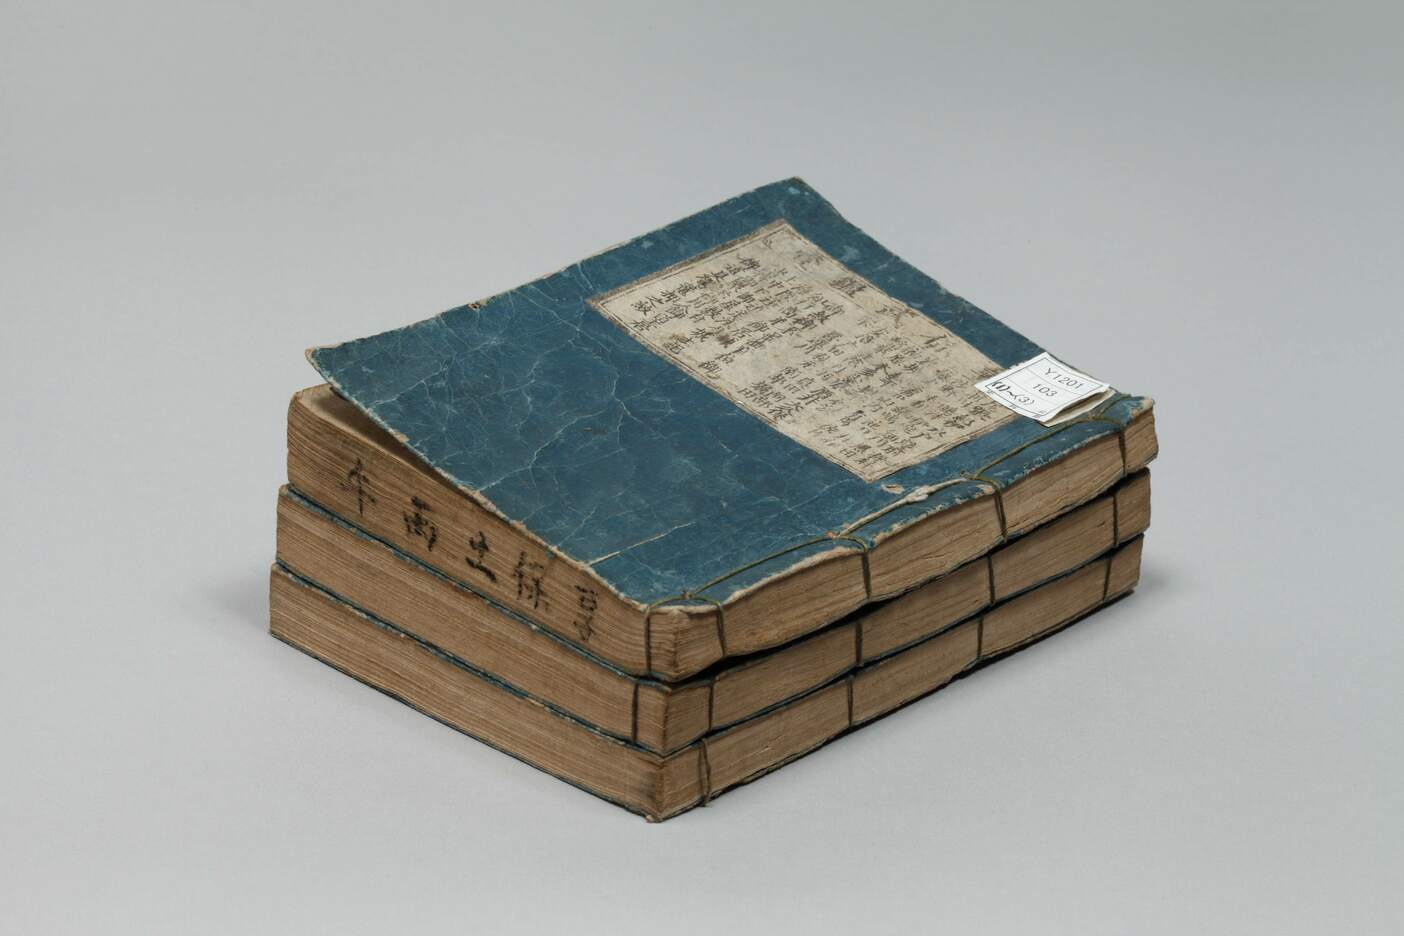
\includegraphics[width=0.7\linewidth]{200018769_00001}
      \caption{Kyōhō Bukan from approx. 1726}
    \end{figure}
  \end{frame}

  \begin{frame}
    \frametitle{Bukan Collection?}
    \framesubtitle{Some more details}
    \begin{columns}
      \begin{column}{.4\linewidth}
        \begin{itemize}
        \item Woodblock-printed
        \item Published 1603-1868
        \item Lists of government officials and other important persons
        \item Written in \alert{pre-modern Japanese}
        \end{itemize}
      \end{column}
      \begin{column}{.6\linewidth}
        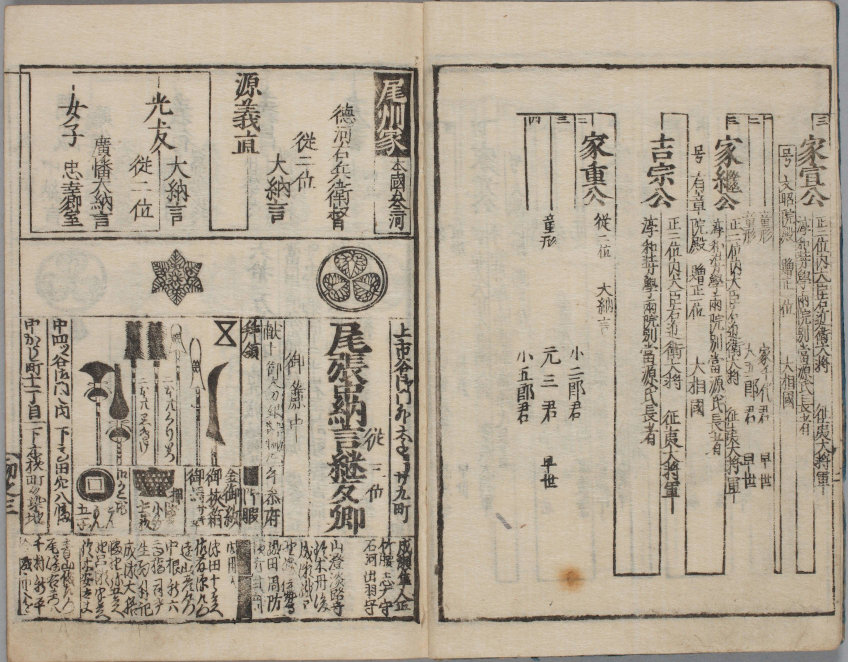
\includegraphics[width=1.0\linewidth]{200018769_00006}
      \end{column}
    \end{columns}
  \end{frame}

  \begin{frame}
    \frametitle{Bukan Collection?}
    \framesubtitle{Statistics}
    \begin{columns}
      \begin{column}{0.4\linewidth}
        \begin{itemize}
        \item 250 scanned book
        \item 90,000 images
        \item Varying quality
        \end{itemize}
      \end{column}
      \begin{column}{.6\linewidth}
        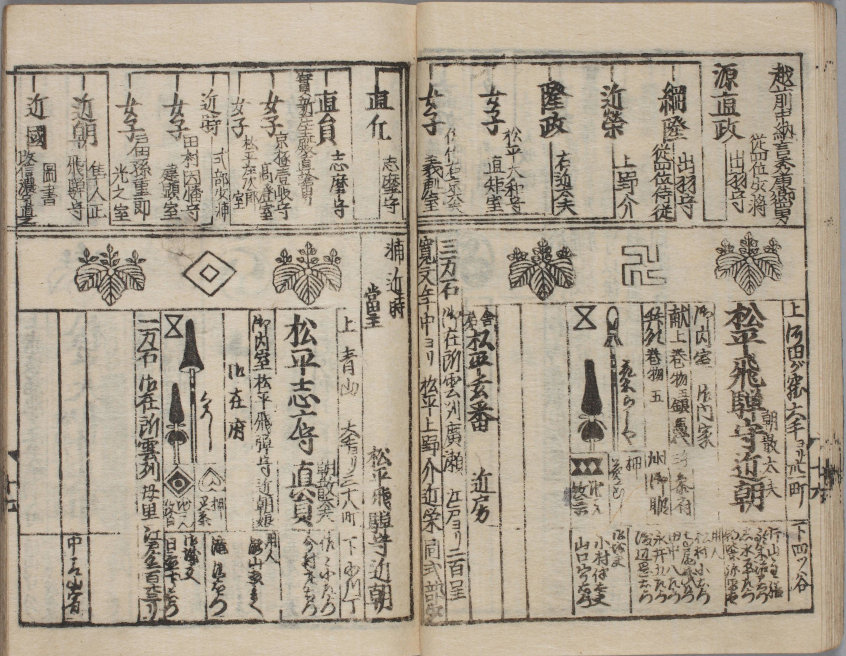
\includegraphics[width=1.0\linewidth]{200018769_00020}
      \end{column}
    \end{columns}
  \end{frame}

  \begin{frame}
    \frametitle{Goals}
    I want to detect if the same woodblock was used in different books. \vspace{0.5em}

    I want to detect and visualize modifications of the woodblock. \vspace{0.5em}
    \begin{figure}
      \centering
      \Huge
      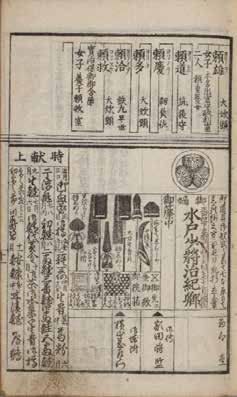
\includegraphics[width=0.2\linewidth]{book1} ↔
      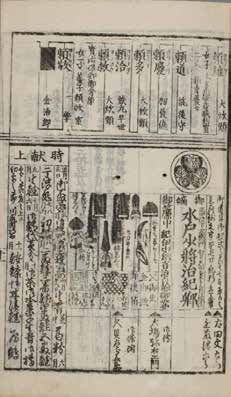
\includegraphics[width=0.2\linewidth]{book2} =
      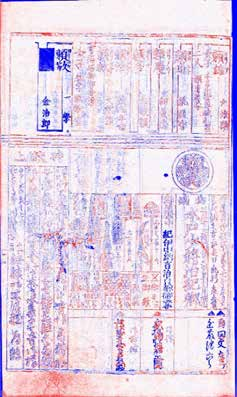
\includegraphics[width=0.2\linewidth]{bookdiff}
      \caption{``Image-Based Change Detection'' (Kitamoto et. al. 2018/6/29)}
    \end{figure}
  \end{frame}

  \begin{frame}
    \frametitle{Approaches}
    \framesubtitle{For detecting same woodblocks}
    Detecting perceptual similar images
    \begin{itemize}
    \item Feature vectors
    \item Perceptual hashes
    \item Features from Deep Autoencoders
    \end{itemize}
    \begin{figure}
      \centering
      \framebox(45,60){Image}
      \Huge→
      \normalsize $\begin{bmatrix} x_1 \\ x_2 \\ \vdots \\ x_n \end{bmatrix}$

      \vspace{1em}Comparing features is faster and more robust than comparing pixels.
    \end{figure}
  \end{frame}
  
  \begin{frame}
    \frametitle{Approaches}
    \framesubtitle{For detecting modifications}
    \begin{itemize}
    \item Feature matching
    \item Appropriate pre-processing
      \begin{itemize}
      \item Thresholding, Aligning, Page detection, …
      \end{itemize}
    \end{itemize}
    \begin{figure}
      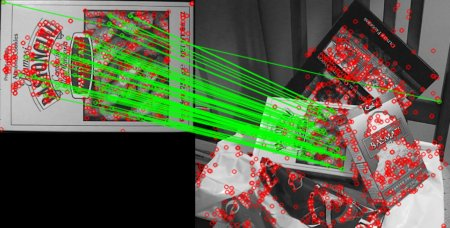
\includegraphics[width=.6\linewidth]{matcher_flann}
      \caption{OpenCV Feature Matching Example}
    \end{figure}
  \end{frame}

\end{document}